                %%%%%%%%%%%%%%%%%%%%%%%%%%%%%%%%%%%%%%%%%
% University Assignment Title Page 
% LaTeX Template
% Version 1.0 (27/12/12)
%
% This template has been downloaded from:
% http://www.LaTeXTemplates.com
%
% Original author:
% WikiBooks (http://en.wikibooks.org/wiki/LaTeX/Title_Creation)
%
% License:
% CC BY-NC-SA 3.0 (http://creativecommons.org/licenses/by-nc-sa/3.0/)
% 
% Instructions for using this template:
% This title page is capable of being compiled as is. This is not useful for 
% including it in another document. To do this, you have two options: 
%
% 1) Copy/paste everything between \begin{document} and \end{document} 
% starting at \begin{titlepage} and paste this into another LaTeX file where you 
% want your title page.
% OR
% 2) Remove everything outside the \begin{titlepage} and \end{titlepage} and 
% move this file to the same directory as the LaTeX file you wish to add it to. 
% Then add \input{./title_page_1.tex} to your LaTeX file where you want your
% title page.
%
%%%%%%%%%%%%%%%%%%%%%%%%%%%%%%%%%%%%%%%%%
%\title{Title page with logo}
%----------------------------------------------------------------------------------------
%   PACKAGES AND OTHER DOCUMENT CONFIGURATIONS
%----------------------------------------------------------------------------------------

\documentclass[12pt]{article}
\usepackage[english]{babel}
\usepackage[utf8x]{inputenc}
\usepackage{amsmath}
\usepackage{graphicx}
\usepackage[colorinlistoftodos]{todonotes}
\usepackage[T1]{fontenc}
\usepackage{listings}
\usepackage{color}


\definecolor{dkgreen}{rgb}{0,0.6,0}
\definecolor{gray}{rgb}{0.5,0.5,0.5}
\definecolor{mauve}{rgb}{0.58,0,0.82}
 
\lstset{
  language=C,                
  basicstyle=\footnotesize,           
  numbers=left,                   
  numberstyle=\tiny\color{gray},  
  stepnumber=2,                             
  numbersep=5pt,                  
  backgroundcolor=\color{white},    
  showspaces=false,               
  showstringspaces=false,         
  showtabs=false,                 
  frame=single,                   
  rulecolor=\color{black},        
  tabsize=2,                      
  captionpos=b,                   
  breaklines=true,                
  breakatwhitespace=false,        
  title=\lstname,                               
  keywordstyle=\color{blue},          
  commentstyle=\color{dkgreen},       
  stringstyle=\color{mauve},     
}


\begin{document}

\begin{titlepage}
\newcommand{\HRule}{\rule{\linewidth}{0.5mm}} % Defines a new command for the horizontal lines, change thickness here

\center % Center everything on the page
 
%----------------------------------------------------------------------------------------
%   HEADING SECTIONS
%----------------------------------------------------------------------------------------

\textsc{\LARGE Universidade Federal do Rio de Janeiro}\\[1.5cm] % Name of your university/college
\textsc{\LARGE Escola Politécnica }\\[1.5cm] % Name of your university/college
\textsc{\Large Departamento de Engenharia Eletrônica e de Computação}\\[0.5cm] % Major heading such as course name
\textsc{\large Projeto Integrado 2017.1}\\[0.5cm] % Minor heading such as course title

%----------------------------------------------------------------------------------------
%   TITLE SECTION
%----------------------------------------------------------------------------------------

\HRule \\[0.4cm]
{ \huge \bfseries Boat Tracker}\\[0.4cm] % Title of your document
\HRule \\[1.5cm]
 
%----------------------------------------------------------------------------------------
%   AUTHOR SECTION
%----------------------------------------------------------------------------------------

\begin{minipage}{0.4\textwidth}
\begin{flushleft} \large
\emph{Autores:}\\
Matheus \textsc{Hoffmann}
William \textsc{Macedo}% Your name
\end{flushleft}
\end{minipage}
~
\begin{minipage}{0.4\textwidth}
\begin{flushright} \large
\emph{Supervisores:} \\
Fábio \textsc{Nascimento\\}
Luiz Felipe \textsc{Moraes\\(LIOc/COPPE/UFRJ)\\}
% Supervisor's Name
Carlos J. R. \textsc{D'ávila\\}
Joarez B. \textsc{Monteiro\\}
(DEL/POLI/UFRJ)% Supervisor's Name
\end{flushright}
\end{minipage}\\[2cm]

% If you don't want a supervisor, uncomment the two lines below and remove the section above
%\Large \emph{Author:}\\
%John \textsc{Smith}\\[3cm] % Your name

%----------------------------------------------------------------------------------------
%   DATE SECTION
%----------------------------------------------------------------------------------------

{ Agosto de 2017}\\[2cm] % Date, change the \today to a set date if you want to be precise

%----------------------------------------------------------------------------------------
%   LOGO SECTION
%----------------------------------------------------------------------------------------


\includegraphics[width=32mm,scale=0.5]{ufrj-logo-9.png}\\[1cm] % Include a department/university logo - this will require the graphicx package
 
%----------------------------------------------------------------------------------------

\vfill % Fill the rest of the page with whitespace

\end{titlepage}


\begin{abstract}
O projeto Boat Tracker consiste n'uma plataforma de monitoramento de posição para embarcações marítimas pequenas.
A plataforma é composta por dois sistemas: Embarcado e de Terra.
O sistema embarcado é composto por um microcontrolador, produzido pela Texas Instruments, MSP432 atuando sobre um sensor GPS - \textit{Sistema de Posicionamento Global} -
e um módulo GSM - \textit{Sistema Global para Comunicações Móveis}.
O sistema de Terra recebe as mensagens do sistema embarcado, via e-mail, com as coordenadas geográficas e a situação da embarcação e armazena em um \textit{Data Logger}.
No final, o sistema de Terra agirá como Host Server e disponibilizará um endereço Web
em que os usuários podem fazer requisição do último dado armazenado e então a página exibe um mapa com essas coordenadas e a situação da embarcação.
< Outras funcionalidades: Rota de ultimas posições, botão emergência, ponto inicial e final>
\end{abstract}

\section{Motivação}
\hspace{0.5cm} A principal motivação do desenvolvimento deste projeto é a necessidade do monitoramento de embarcações ao longo de competições de pequeno porte.
Um problema recorrente no ambiente competitivo marítmo é que tanto os espectadores quanto as equipes em terra não conseguem avaliar, sem ajuda de instrumentos de medição, o ranqueamento das embarcações no momento atual do evento. A primeira aplicação para o projeto tem como inspiração o projeto da Federação Brasiliense de Vela Adaptada, oferecendo às pessoas com deficiência a possibilidade de praticar um esporte, resgatar a autoestima e melhorar a qualidade de vida. A idéia é trazer esse projeto para o Rio de Janeiro e usar o protótipo do projeto. O Laboratório de Instrumentação Oceanográfica da COPPE/UFRJ é apoiador deste projeto, e também dá suporte para a realização deste projeto integrado. Seus autores são bolsistas de iniciação científica do referido laboratório.

\section{Introdução}
\hspace{0.5cm} O projeto começa no módulo GPS, ele capta as informações de longitude e latitude no presente momento bem como data, hora e velocidade absoluta. Cabe ao microcontrolador MSP432 guardar essa informação e enviar o mais rápido possível via e-mail usando o módulo GSM. A partir disso o sistema de terra possui um script em Python que verifica indefinidamente a existência de novos e-mails na caixa de entrada, valida de acordo com o remetente e armazena a informação em um Data Logger diário. Por fim a interface web, via PHP, seleciona dentre os arquivos de logs diários no servidor o último modificado, portanto o dia atual recente e carrega a última aquisição desse dia do tracker para a API do Google Maps.

\section{Precificação}
\begin{itemize}
\item Módulo GPS/GSM SIM808 - R\$155,00
\end{itemize}
\begin{itemize}
\item Microcontrolador Texas Instruments Launchpad MSP432P401R - R\$ 45,00
\end{itemize}
\begin{itemize}
\item Alimentação Elétrica + Cabeamento - R\$30,00
\end{itemize}
\begin{itemize}
\item Caixa Patola - R\$ 20,00
\end{itemize}

Total: R\$250,00
Observação: Todo o projeto foi custeado pelo LIOc/COPPE/UFRJ

\section{Sistema Embarcado}

\subsection{Descrição do Funcionamento}
\hspace{0.5cm} O Sistema embarcado é composto por duas partes (placas) principais. A primeira é o módulo que contém o chip SIM808. Este chip integra diversas de função de comunicações móveis (2G - GPRS/GSM), geolocalização (GPS/GNSS) e comunicações locais (Bluetooth). Para a nossa aplicação, utilizaremos suas funções de comunicação móvel e geolocalização. Sua escolha foi motivada após pesquisa de diversos chips, que aliassem os seguintes fatores: baixo custo, facilidade de programação, documentação vasta e rápido tempo de aquisição (compra em território nacional). A segunda parte é a placa controladora, o cérebro do sistema, o microcontrolador MSP432P401R, fabricado pela renomada Texas Instruments. Sua escolha foi motivada principalmente pelo uso constante dos microcontroladores da família MSP430/MSP432 pelos alunos desenvolvedores e pesquisadores do LIOc. Suas principais características são: extremo baixo consumo, disponibilidade de interfaces de comunicação (SPI/I2C/UART) e programação em C. Diversas outras características fazem o LIOc ter adotado tal placa como referência em diversos de seus projetos e de seus integrantes (projetos finais de graduação e dissertações de mestrado), porém não são do escopo deste projeto integrado.

A placa controladora se comunica com o módulo através do protocolo serial UART (assíncrono), e utilizando do protocolo AT, de comunicações móveis. São enviados comandos básicos, como: ligue o seu módulo GPRS, ligue o seu módulo GPS e transmita informação de GPS para sua saída. A string com a localização GPS é obtida pelo microcontrolador, que "parsea" esta informação, e envia de volta para o módulo, solicitando que um e-mail seja enviado para o servidor (sistema web). 

O consumo médio deste módulo é de 100mA, com picos de 250mA nas transmissões para a ERB da rede celular. 
O consumo da placa controladora reside na faixa de 5mA, porém com otimizações, este valor pode cair para a região das centenas de microAmperes.

\begin{figure}[h]
\caption{Diagrama de Funcionamento do Sistema Embarcado}

\centering % para centralizarmos a figura
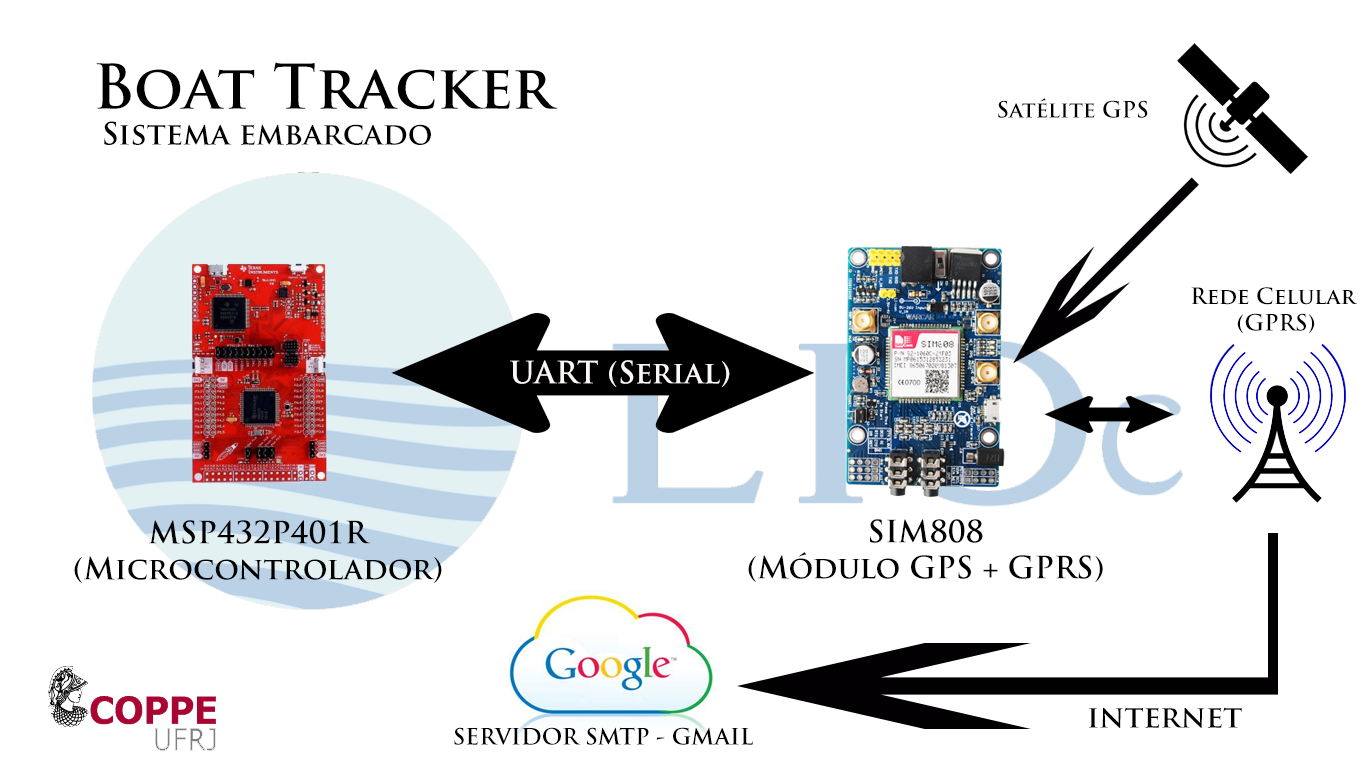
\includegraphics[width=12cm]{Diagrama_Funcionamento_Sist_Emb.png} % leia abaixo
\label{figura:qualquernome}
\end{figure}

\subsection{Plataforma de Desenvolvimento}
\hspace{0.5cm} Para a realização da codificação do microcontrolador, utilizou-se a IDE (Integrated Development Enviroment) Energia. Esta IDE é baseada na IDE nativa do Arduino. O principal motivo pelo qual se optou pela Energia foi a possibilidade de programação em mais alto nível, em comparação com a linguagem C ANSI. No Energia, utiliza-se uma linguagem muito similar a C++, permitindo que operações como transmissão e recepção UART e parsing de strings GPS fossem realizados com mais facilidade. Dessa forma, menos tempo foi desprendido em programação de baixo nível. Segue o código principal abaixo:



\begin{verbatim}

/* DEL/POLI/UFRJ
   Projeto Integrado 2017.1
   Código Fonte - Sistema Embarcado
   Autores:
   William Barbosa de Macedo - william.macedo@poli.ufrj.br
   Matheus Hoffmann Fernandes Santos - hoffmann@poli.ufrj.br

*/
#include "auxiliares.h"
#define DEBUG true
#define EMERGENCIA 10

/* Declaração de Variáveis/Objetos */
//TinyGPSPlus gps;         // Objeto GPS
char gprmc[100];
String mensagem, telefone;
int status;

void sendSMS(String mensagem);
void goGPS(void);
void go2G(void);      // setar APN da operadora
void lerSerial(void); // testar
void sendEmail(String);
void sendData(String, const int, boolean);

void setup()   /* Essa rotina é executada apenas uma vez */
{
    Serial.begin(9600);   /* abre a porta serial de comunicação entre 
o MSP432 e o PC. Será útil para enviar informações de debug ao Serial Monitor */
    Serial1.begin(9600);  /* abre a porta serial de comunicação entre 
o MSP432 e o Módulo GSM/GPS */
    pinMode(RED_LED, OUTPUT);
    pinMode(GREEN_LED, OUTPUT);
    pinMode(BLUE_LED, OUTPUT);
    status = pinMode(EMERGENCIA, INPUT);
    digitalRead(EMERGENCIA);
    comandoAT("AT");                              // sim808, are you alive?
    delay(10000);         /* Delay para fixação da Rede GPRS 
(Nextel no LIOc - por volta de 15s */
    sendData( "AT+CGPSPWR=1",1000,DEBUG);
    sendData( "AT+CGNSPWR=1",1000,DEBUG);
    sendData( "AT+CGPSOUT=255",1000,DEBUG);
    sendData( "AT+CGNSTST=1",1000,DEBUG);
    sendData( "",1000,DEBUG);
    sendData( "",1000,DEBUG);
    sendData( "",1000,DEBUG);
    //sendData( "AT+CGPSPWR=0",1000,DEBUG);
    go2G();                                       // configura e ativa GPRS
    sendEmail(gprmc);
}

void loop()   /* Loop principal do programa. Executado após o setup */
{
  go2G();                                       // configura e ativa GPRS
  sendData( "AT+CGPSPWR=1",1000,DEBUG);
  sendData( "AT+CGPSOUT=255",1000,DEBUG);
  sendData( "AT+CGNSTST=1",1000,DEBUG);
  status = digitalRead(EMERGENCIA);
  char(status);
  sendData( "",1000,DEBUG);
  sendData( "",1000,DEBUG);
  gprmc += '\n';
  gprmc += status;
  sendEmail(gprmc);
}

void sendSMS(String mensagem)
{
    comandoAT("AT+CMGF=1");
    comandoAT("AT+CMGS=\"00000000000\"");
    Serial1.print(mensagem);
    delay(500);
    ctrlZ();
}

void lerSerial(void)
{
  String respostaAT;

  respostaAT = "";
  while(Serial1.available() > 0) // aguarda recebimento de mensagem de 
//confirmacao. Quando for -1, indica que não há mais dados a serem processados.
  {
    char c = Serial1.read();
    respostaAT += c; // le mensagem recebida. 
// Concatena os chars em uma string. Typecast pq read retorna int.
  }

  if (respostaAT.length() >0)
  {
    Serial.print("Leitura Serial: ");
    Serial.println(respostaAT);
  }
}

void goGPS(void)
{
  comandoAT("AT+CGNSPWR=1");
  comandoAT("AT+CGNSTST=1");
}

void go2G(void)
{
  comandoAT("AT+SAPBR=3,1,\"Contype\",\"GPRS\"");   
// APN ou Contype
  comandoAT("AT+SAPBR=3,1,\"APN\",\"modem.nextel3g.net.br\"");  
 // atencao: trocar APN para sua respectiva operadora
  comandoAT("AT+SAPBR=1,1");
  comandoAT("AT+SAPBR=2,1");
}

void sendEmail(String mensagem)
{
  comandoAT("AT+EMAILCID=1");
  comandoAT("AT+EMAILTO=45");
  comandoAT("AT+EMAILSSL=2");
  comandoAT("AT+SMTPSRV=\"smtp.gmail.com\",25");
  comandoAT("AT+SMTPAUTH=1,\"lioc.boat.tracker@gmail.com\",\"REMOVED\"");
  comandoAT("AT+SMTPFROM=\"lioc.boat.tracker@gmail.com\",\"TRACKER01\"");
  comandoAT("AT+SMTPRCPT=0,0,\"lioc.boat.tracker@gmail.com\",\"Server\"");
  comandoAT("AT+SMTPRCPT=1,0,\"william.macedo@poli.ufrj.br\",\"William\"");
  comandoAT("AT+SMTPSUB=\"BT01\"");
  comandoAT("AT+SMTPBODY=70");
  comandoAT(mensagem);
  ctrlZ();
  comandoAT("AT+SMTPSEND");
  delay(15000);
}

void sendData(String command, const int timeout, boolean debug){
    String response = "";

    Serial1.println(command);
    delay(150);
    if(debug){
    long int time = millis();
    while( (time+timeout) > millis()){
      while(Serial1.available()){
        response += char(Serial1.read());
      }
    }
//      Serial.println("\nInicio da Resposta");
//      Serial.print(response);
//      Serial.println("\nFim da Resposta");
    int index=0, indice=0;
      index = response.indexOf("$GPRMC",0);  // if(index != -1)
      if(index >=0)
      {
        time = millis();
        do
        {
          gprmc[indice] = response[index];
          indice++;
          index++;
          if(indice==95)
            break;
        }
        while((response[index] != '$') && ((time+timeout) > millis()));

        //gprmc[indice] = '\0';
        Serial.println("\Inicio do GPRMC:");
        Serial.print(gprmc);
        Serial.println("Fim do GPRMC\n");
      }
    }
}

\end{verbatim}

\subsection{Principais dificuldades}
\hspace{0.5cm} Houve bastante dificuldade para realizar o recebimento de forma adequada da string proveniente do módulo GPS. Isso se dá ao fato de que o buffer do MSP432 é de apenas 32 bytes. De início, a codificação não estava adequada, e os bytes subsequentes ao trigésimo segundo eram perdidos. O código atual resolve este problema. Também houveram desafios no que tange ao envio do e-mail. O servidor SMTP do Google, que realiza os Log-Ins e permite o acesso ao endereço de e-mail, apenas responde a conexões que estejam protegidas pelo protocolo de segurança SSL. Para enviar uma mensagem com este protocolo, se fez necessário atualização do Firmware do módulo GPRS, através de uma conexão serial com o Notebook. Outra questão observada foi o fato de que, após ligado, o módulo
GPS envia dados ininterruptamente ao microcontrolador, dos mais diversos tipos de formatos NMEA (GPRMC, GPGGA etc). Entretanto, apenas o protocolo GPRMC era de fato, o interesse de ser adquirido. Para tal, se fez necessário a detecção assíncrona dos caracteres de identificação do protocolo e dos caracteres iniciais "G; P; R; M e C" conforme o buffer tinha o seu preenchimento. 

\subsection{Entendimento do Sistema - Desenvolvedor}
\hspace{0.5cm} Os códigos do sistema embarcado estão armazenados no repositório oficial do Boat Tracker: https://github.com/Hoffmannxd/BoatTracker. Todos os arquivos estão documentados e comentados. A maioria das funções utilizadas são auto-explicativas e seguem as recomendações dos desenvolvedores do módulo GPS/GPRS. Os comandos AT são utilizados,em sua maioria, na sequência que é exemplificada no manual do módulo (SIM808), para cada procedimento (enviar e-mail, ligar GPRS etc). Dúvidas que não forem sanadas ao ler os comentários, ou ao ler os arquivos de orientação do módulo SIM808 (disponíveis na Internet), podem ser sanadas contatando william.macedo@poli.ufrj.br.

\section{Sistema de Terra - Detalhamento}

\hspace{0.5cm} O Sistema de terra foi concebido em um Notebook Asus, com processador Intel i5. Neste notebook foi instalado um Servidor (Apache). Um código em python é responsável por checar o e-mail para o qual o sistema embarcado envia as informações de geolocalização. A cada novo e-mail que é detectado pelo sistema, este programa recebe a string GPRMC (um dos padrões internacionais para informação de geolocalização - via satélite), e as parsea novamente, para obter os valores finais de longitude e latitude. Exemplo de String GPRMC: \\ \\ \$GPRMC,153421.000,A,2251.6658,S,04313.7370,W,0.01,120.76,030717,,,A*6F \\

Esta string aponta para o corredor do Centro de Tecnologia da UFRJ. Dado obtido ás 12:34 - UTC-3 (15:34 - UTC) do dia 03/07/2017. No momento da aquisição, o autor estava almoçando em um dos trailers do CT. Para rápida visualização, copie e cole a string no site: https://rl.se/gprmc

Após a obtenção destes valores, um arquivo de LOG é criado para registrar esta ocorrência de rastreamento. Um programa em PHP, que roda no servidor Apache, também recebe estes valores, e , com auxílio de uma API fornecida pelo Google Maps, plota essas informações em um Mapa, onde podemos visualizar claramente a posição do sistema embarcado, no momento da aquisição.

\subsection{Qualidade das Medidas e Observações}
\hspace{0.5cm} Para medidas em ceú aberto, foram realizados ensaios (inclusive com chuva), que nos resultaram em localizações com exatidão inferior a 2m. Ao adentrar em ambiente fechado (salas e auditórios), a precisão e exatidão das medidas vão se reduzindo, até que o sinal dos satélites é perdido completamente (inerente da baixa potência que chega à superfície da terra, advinda da órbita terrestre). O Sinal de GPRS varia conforme a operadora utilizada. Em todos os nossos testes utilizamos a rede da operadora NEXTEL. Considerando a baixa qualidade média de sinal celular em toda a Ilha do Fundão, onde o sistema foi testado, consideramos que o nosso objetivo foi alcançado com sucesso.

\section{Projetos Futuros}
\hspace{0.5cm} Como citado anteriormente, este projeto integrado é o início de um projeto em andamento do LIOc/COPPE/UFRJ. Há um planejamento para continuação do desenvolvimento para aplicação em uma competição que deve ocorrer no final deste ano (2017). As principais melhorias a serem feitas são: Aprimoramento do encapsulamento, cabeamento e alimentação. Redução máxima do consumo do sistema, otimização de todos os códigos, com processos mais eficientes, redução do tempo de atualização da localização (atualmente na região de 40 segundos, com bom sinal de 2G) e redução de custos. Também há a possibilidade da mudança da forma como o dado navega pela rede de internet (atualmente - E-mail/Google). Uma das possibilidades é a montagem de um servidor FTP, reduzindo o caminho até a máquina de destino.

\section{Agradecimentos}
\hspace{0.5cm} Agradecemos imensamente aos Professores Carlos José Ribas D'ávila (Casé) e Joarez Bastos Monteiro pela ministração desta disciplina, a qual consideramos uma das mais importantes do curso de Engenharia Eletrônica e de Computação da UFRJ. Agradecemos também aos Engenheiros Fábio Nascimento pela concepção da ideia e motivação, e Luiz Felipe Moraes por toda a ajuda técnica com sua experiência na área de sistemas embarcados.\\\\Contatos:\\William Barbosa de Macedo -   william.macedo@poli.ufrj.br\\Matheus Hoffmann Fernandes Santos - hoffmann@poli.ufrj.br

\end{document}
